\documentclass[12pt]{article}

\usepackage[margin=1in]{geometry}
\usepackage{fancyhdr}
\usepackage{longtable}
\usepackage{array}
\usepackage{hyperref}
\usepackage{enumitem}
\usepackage{titlesec}
\usepackage{xcolor}
\usepackage{graphicx}
\usepackage{tikz}
\usetikzlibrary{arrows.meta, positioning, shapes.geometric}

\hypersetup{
    colorlinks=true,
    linkcolor=blue,
    urlcolor=blue
}

\pagestyle{fancy}
\fancyhf{}
\lhead{Software Design Document}
\rhead{Product Expiration Tracking App}
\cfoot{\thepage}

\title{Software Design Document (SDD)\\Product Expiration Tracking Application}
\author{Prepared for Course Project}
\date{\today}

\begin{document}

\maketitle
\newpage
\tableofcontents
\newpage

\section*{Document Revision History}
\addcontentsline{toc}{section}{Document Revision History}

\begin{longtable}{|p{0.15\textwidth}|p{0.18\textwidth}|p{0.22\textwidth}|p{0.35\textwidth}|}
\hline
\textbf{Version} & \textbf{Date} & \textbf{Snapshot} & \textbf{Description of Revision} \\
\hline
0.1 & Snapshot 1 & Initial Design & Created the first high-level architecture and identified frontend, backend, database, and notification components. \\
\hline
0.2 & Snapshot 2 & Detailed Design & Added module descriptions, data design, API design, and screen design. \\
\hline
0.3 & Snapshot 3 & Design Refinement & Updated the design to use React Native for the mobile client and Node.js for the backend REST API. \\
\hline
1.0 & Final Snapshot & Final Submission & Completed final design, including security, error handling, deployment, testing, and future design considerations. \\
\hline
\end{longtable}

\section{Introduction}

\subsection{Purpose}
This Software Design Document (SDD) describes the architecture and technical design of a product expiration tracking application. The application uses a React Native frontend for mobile devices and a Node.js backend for application logic, authentication, and data access. The purpose of this document is to explain how the system will be built based on the requirements defined in the SRS.

\subsection{Scope}
The design covers the mobile frontend, backend API, database design, authentication flow, product tracking logic, notification handling, and deployment approach. The first version focuses on manual product entry, expiration tracking, search/filtering, and reminders.

\subsection{Design Goals}
\begin{itemize}
    \item Provide a simple and user-friendly mobile experience.
    \item Keep the backend modular and maintainable.
    \item Protect user data through secure authentication and authorization.
    \item Support future features such as barcode scanning, AI recognition, family sharing, and offline mode.
    \item Make the system easy to test and deploy.
\end{itemize}

\section{System Overview}

\subsection{High-Level Architecture}
The system follows a client-server architecture. The React Native mobile application sends HTTPS requests to the Node.js backend API. The backend validates requests, applies business logic, and stores or retrieves data from the database. A notification service or scheduled backend process checks expiration dates and prepares reminders.

\begin{center}
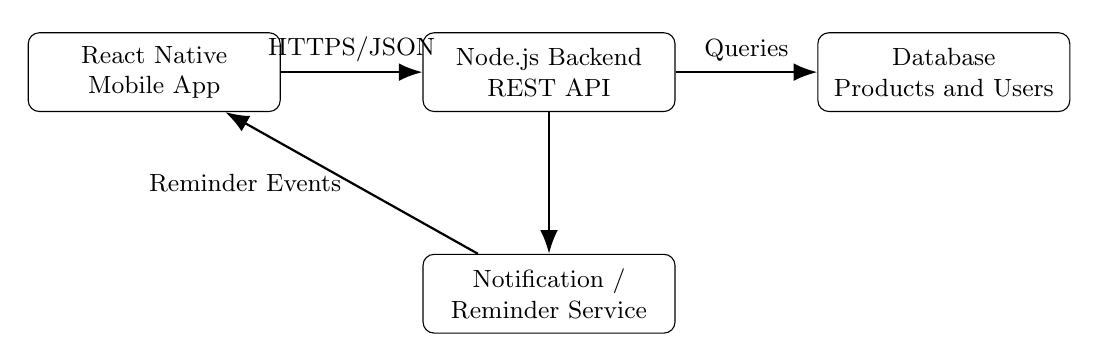
\begin{tikzpicture}[
    node distance=1.8cm,
    every node/.style={font=\small},
    box/.style={rectangle, draw, rounded corners, minimum width=3.2cm, minimum height=1cm, align=center},
    arrow/.style={-{Latex[length=3mm]}, thick}
]

\node[box] (mobile) {React Native\\Mobile App};
\node[box, right=of mobile] (api) {Node.js Backend\\REST API};
\node[box, right=of api] (db) {Database\\Products and Users};
\node[box, below=of api] (notify) {Notification /\\Reminder Service};

\draw[arrow] (mobile) -- node[above]{HTTPS/JSON} (api);
\draw[arrow] (api) -- node[above]{Queries} (db);
\draw[arrow] (api) -- (notify);
\draw[arrow] (notify) -- node[left]{Reminder Events} (mobile);

\end{tikzpicture}
\end{center}

\subsection{Technology Stack}
\begin{longtable}{|p{0.28\textwidth}|p{0.62\textwidth}|}
\hline
\textbf{Layer} & \textbf{Technology / Design Choice} \\
\hline
Mobile Frontend & React Native with JavaScript or TypeScript. The app supports iOS and Android devices. \\
\hline
Backend & Node.js with Express.js or a similar framework for REST API development. \\
\hline
Database & PostgreSQL, MongoDB, or another suitable database. For this design, PostgreSQL is recommended because the data has clear relationships between users, products, categories, and reminders. \\
\hline
Authentication & JWT-based authentication with hashed passwords. \\
\hline
Notifications & Mobile push notifications using platform services or a service such as Firebase Cloud Messaging. \\
\hline
Deployment & Backend hosted on a cloud server or platform. Mobile app distributed through development builds or app stores. \\
\hline
\end{longtable}

\section{Architectural Design}

\subsection{Frontend Architecture}
The React Native frontend is organized into screens, reusable components, navigation, API services, state management, and utility functions. This separation keeps the mobile code easier to maintain and test.

\begin{longtable}{|p{0.28\textwidth}|p{0.62\textwidth}|}
\hline
\textbf{Frontend Module} & \textbf{Responsibility} \\
\hline
Screens & Full pages such as Login, Register, Dashboard, Product List, Product Detail, Add Product, Edit Product, and Settings. \\
\hline
Components & Reusable UI parts such as ProductCard, ExpirationBadge, CategoryFilter, DatePickerField, and EmptyState. \\
\hline
Navigation & Handles movement between screens using stack and tab navigation. \\
\hline
API Service & Contains functions for calling backend endpoints and handling responses. \\
\hline
State Management & Stores authentication state, product lists, loading states, and user preferences. \\
\hline
Utilities & Helper functions for date formatting, expiration calculations, validation, and error display. \\
\hline
\end{longtable}

\subsection{Backend Architecture}
The Node.js backend is organized into routes, controllers, services, models, middleware, and configuration files.

\begin{longtable}{|p{0.28\textwidth}|p{0.62\textwidth}|}
\hline
\textbf{Backend Module} & \textbf{Responsibility} \\
\hline
Routes & Define API endpoints and connect requests to controllers. \\
\hline
Controllers & Receive HTTP requests, validate input, call services, and return responses. \\
\hline
Services & Contain business logic, such as expiration classification and reminder scheduling. \\
\hline
Models / Data Access & Define database tables or schemas and perform database operations. \\
\hline
Middleware & Handle authentication, authorization, error handling, request logging, and validation. \\
\hline
Configuration & Store environment-specific settings such as database URL, JWT secret, and notification settings. \\
\hline
\end{longtable}

\section{Detailed Component Design}

\subsection{Authentication Component}
The authentication component manages registration, login, password hashing, and token generation. When a user registers, the backend validates the input and stores a hashed password. When a user logs in, the backend compares the submitted password with the stored hash. If the credentials are valid, the backend returns a JWT. The mobile app stores the token securely and includes it in future API requests.

\subsection{Product Management Component}
The product management component handles creating, reading, updating, and deleting product records. Each product belongs to one user. The backend checks the authenticated user ID before returning or modifying product data. This prevents users from accessing another user's products.

\subsection{Expiration Tracking Component}
The expiration tracking component calculates the status of each product. A product can have one of the following statuses:
\begin{itemize}
    \item \textbf{Expired}: expiration date is before the current date.
    \item \textbf{Soon to Expire}: expiration date is within the user's reminder period.
    \item \textbf{Safe}: expiration date is later than the reminder period.
\end{itemize}

\subsection{Reminder Component}
The reminder component checks products that are close to expiration and creates notification events. In the first version, reminders may be calculated when the dashboard loads. In a more advanced version, a scheduled backend job can run daily and send push notifications.

\subsection{Search and Filtering Component}
The search and filtering component allows the user to search by product name and filter by category, location, or expiration status. Sorting by expiration date helps users see urgent items first.

\section{Data Design}

\subsection{Database Tables}
This design recommends a relational database structure. The exact SQL syntax may change depending on the database and library used.

\subsubsection{Users Table}
\begin{longtable}{|p{0.25\textwidth}|p{0.25\textwidth}|p{0.4\textwidth}|}
\hline
\textbf{Field} & \textbf{Type} & \textbf{Description} \\
\hline
id & UUID / Integer & Unique user identifier. \\
\hline
name & String & User's display name. \\
\hline
email & String & Unique email address. \\
\hline
password\_hash & String & Securely hashed password. \\
\hline
notification\_enabled & Boolean & Indicates whether reminders are enabled. \\
\hline
reminder\_days & Integer & Number of days before expiration to remind the user. \\
\hline
created\_at & Timestamp & Account creation time. \\
\hline
updated\_at & Timestamp & Last update time. \\
\hline
\end{longtable}

\subsubsection{Products Table}
\begin{longtable}{|p{0.25\textwidth}|p{0.25\textwidth}|p{0.4\textwidth}|}
\hline
\textbf{Field} & \textbf{Type} & \textbf{Description} \\
\hline
id & UUID / Integer & Unique product identifier. \\
\hline
user\_id & UUID / Integer & Owner of the product. \\
\hline
name & String & Product name. \\
\hline
category & String & Product category. \\
\hline
expiration\_date & Date & Product expiration date. \\
\hline
quantity & String / Integer & Product amount or count. \\
\hline
location & String & Storage location. \\
\hline
notes & Text & Optional user notes. \\
\hline
image\_url & String & Optional product image path or URL. \\
\hline
created\_at & Timestamp & Product creation time. \\
\hline
updated\_at & Timestamp & Last product update time. \\
\hline
\end{longtable}

\subsubsection{Reminders Table}
\begin{longtable}{|p{0.25\textwidth}|p{0.25\textwidth}|p{0.4\textwidth}|}
\hline
\textbf{Field} & \textbf{Type} & \textbf{Description} \\
\hline
id & UUID / Integer & Unique reminder identifier. \\
\hline
user\_id & UUID / Integer & Owner of the reminder. \\
\hline
product\_id & UUID / Integer & Product connected to the reminder. \\
\hline
reminder\_date & Date & Date when reminder should be sent. \\
\hline
status & String & Pending, sent, failed, or cancelled. \\
\hline
created\_at & Timestamp & Reminder creation time. \\
\hline
\end{longtable}

\section{API Design}

\subsection{Authentication API}
\begin{longtable}{|p{0.16\textwidth}|p{0.32\textwidth}|p{0.42\textwidth}|}
\hline
\textbf{Method} & \textbf{Endpoint} & \textbf{Description} \\
\hline
POST & /api/auth/register & Creates a new user account. \\
\hline
POST & /api/auth/login & Authenticates a user and returns a JWT. \\
\hline
GET & /api/auth/me & Returns the currently authenticated user's profile. \\
\hline
\end{longtable}

\subsection{Product API}
\begin{longtable}{|p{0.16\textwidth}|p{0.32\textwidth}|p{0.42\textwidth}|}
\hline
\textbf{Method} & \textbf{Endpoint} & \textbf{Description} \\
\hline
GET & /api/products & Returns products owned by the authenticated user. \\
\hline
POST & /api/products & Creates a new product. \\
\hline
GET & /api/products/:id & Returns one product by ID. \\
\hline
PUT & /api/products/:id & Updates an existing product. \\
\hline
DELETE & /api/products/:id & Deletes a product. \\
\hline
\end{longtable}

\subsection{Settings and Reminder API}
\begin{longtable}{|p{0.16\textwidth}|p{0.32\textwidth}|p{0.42\textwidth}|}
\hline
\textbf{Method} & \textbf{Endpoint} & \textbf{Description} \\
\hline
GET & /api/settings & Returns user settings. \\
\hline
PUT & /api/settings & Updates notification and reminder preferences. \\
\hline
GET & /api/reminders & Returns upcoming reminder information. \\
\hline
\end{longtable}

\section{User Interface Design}

\subsection{Main Screens}
\begin{longtable}{|p{0.25\textwidth}|p{0.65\textwidth}|}
\hline
\textbf{Screen} & \textbf{Design Description} \\
\hline
Welcome Screen & Shows the application name, short description, and buttons for login and registration. \\
\hline
Login Screen & Allows users to enter email and password. Shows validation errors when needed. \\
\hline
Dashboard Screen & Shows summary cards for expired products, soon-to-expire products, and total products. \\
\hline
Product List Screen & Displays all products using product cards with name, category, location, and expiration status. \\
\hline
Add/Edit Product Screen & Provides a form for product name, expiration date, category, quantity, location, notes, and optional image. \\
\hline
Product Detail Screen & Shows all details for one product and includes edit/delete actions. \\
\hline
Settings Screen & Allows users to update reminder days, notification preference, and profile information. \\
\hline
\end{longtable}

\subsection{Mobile UX Principles}
The mobile design should use clear labels, large touch targets, simple navigation, and readable status indicators. Expired products should be easy to identify. Soon-to-expire items should appear near the top of the list when sorted by expiration date.

\section{Security Design}

\subsection{Authentication and Authorization}
The backend uses JWT-based authentication. Protected endpoints require a valid token. The token contains the user's ID and expiration time. Authorization checks ensure that users can only access their own records.

\subsection{Password Protection}
Passwords are never stored directly. The backend uses a secure hashing library before saving passwords to the database. During login, the submitted password is compared against the stored hash.

\subsection{Input Validation}
The backend validates all incoming data. Product names, dates, categories, and quantities must meet expected formats. Invalid requests return clear error messages without exposing internal server details.

\section{Error Handling Design}

\subsection{Frontend Error Handling}
The mobile application displays friendly messages for invalid input, failed login, expired sessions, server errors, and network problems. Loading indicators are shown while API requests are in progress.

\subsection{Backend Error Handling}
The backend uses centralized error handling middleware. Errors are logged on the server, while the client receives a safe response with an HTTP status code and a short message.

\section{Deployment Design}

\subsection{Development Environment}
During development, the React Native app may run through a local simulator or physical device. The Node.js backend may run locally. The database may run locally or in a development cloud environment.

\subsection{Production Environment}
In production, the backend should be hosted on a reliable cloud platform. Environment variables should store secrets and configuration values. The application should use HTTPS. The database should have backup and recovery options.

\section{Testing Design}

\subsection{Unit Testing}
Unit tests should verify backend services, expiration calculations, validation logic, and frontend utility functions.

\subsection{API Testing}
API tests should verify authentication, product CRUD operations, authorization rules, and error handling.

\subsection{UI Testing}
UI testing should verify that the main screens display correctly and that users can complete common flows such as registering, logging in, adding a product, and viewing expiration status.

\subsection{Acceptance Testing}
Acceptance testing should confirm that the system satisfies the main requirements in the SRS. Test cases should include valid and invalid input, expired products, soon-to-expire products, and multiple users.

\section{Design Tradeoffs}

\subsection{Manual Entry First}
The first version uses manual product entry because it is simpler and more reliable for an initial project. Barcode scanning and AI recognition can be added later after the core tracking system is stable.

\subsection{Relational Database Choice}
A relational database is recommended because the system has structured data and clear relationships. However, MongoDB could also be used if the project team prefers flexible document storage.

\subsection{Online-First Design}
The first version assumes internet access for backend synchronization. Offline support would improve usability but adds complexity around local storage and data synchronization.

\section{Future Design Improvements}
Future versions may add barcode scanning, AI product recognition, shared household accounts, offline mode, grocery list generation, recipe suggestions, and analytics. The system should remain modular so these features can be added without rewriting the main application.

\section{Conclusion}
This SDD explains how the product expiration tracking application will be designed and implemented. The design uses React Native for the mobile frontend, Node.js for the backend, a secure authentication system, and a database for persistent product storage. The architecture supports the current project requirements while leaving room for future improvements.

\end{document}
